\section{Programmering}
\subsection{Kodestandarder}
\label{Kodestandarder}

Før vi havde kodet en eneste linje kode, havde vi en kodestandard på plads.
Uden en kodestandard kan koden hurtigt gå hen og blive uoverskuelig.
Ligeledes er kodestandarder en effektiv måde at lave kvalitetssikring på selve koden, da det giver nogle meget overskuelige og håndgribelige krav at gå ud fra.
I vores projekt har der ikke været den største diskussion om, hvad kodestandarderne skulle være, da vi alle er meget enige om, at den standard, der bliver sat af Microsoft selv, er god\cite{microsoftcsharp}. 
Vi har ikke haft problemer med, at vi ikke har overholdt kodestandarderne, men de har været med til at give folk et sted at starte, når vi laver kode-review. Se afsnit \ref{versionstyring} for en uddybning af kodereviews.

\subsection{Test-driven development(TDD)}
\label{TDD}

Vi blev enige om, at vi ville prøve at køre TDD.
Vi var alle til et foredrag afholdt af Carlos Cunha fra Polytechnic Institute of Viseu, School of Technology, der omhandlede TDD, og vi synes det var en spændende tilgangsvinkel til softwareudvikling.
Derudover har det at skrive tests været en fælles svaghed for os alle i løbet af første studieår, og vi så det som en god måde at blive bedre til det.

Idéen med TDD er, at man skriver tests, der beskriver den ønskede funktionalitet, inden man implementere funktionaliteten.
Testsne er skrevet ud fra en klasses offentligt tilgængelige snitflade.
Fokusset er på en klasses opførsel, ikke dens implementering.

Metodikken ved TDD er:
Hurtigt skriv en test, kør alle tests og se den nye test fejle, lav en lille ændring i ens program, kør alle tests og se dem alle bestå, refaktorer til at undgå duplikeret kode, sikr at alle tests stadig består.

En stor gevinst ved TDD er, at du er sikker på, at du har tests, der dokumenterer dit systems funktionalitet, så når der laves ændringer og refaktoreringer, er du sikker på, at programmet stadig virker som ønsket.

På figur \ref{fig:TDD} kan ses et eksempel på en testmetode.
Denne test sikrer, at vores client klasse arver fra vores user klasse.

\begin{figure}[H]
    \caption{Eksempel på en unit test}
    \centering
        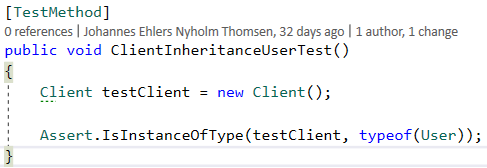
\includegraphics[width=\textwidth]{TestEksempelInheritance.png}
    \label{fig:TDD}
\end{figure}

TDD fungerede rigtig godt for os i de to første sprints, hvor programmets grundstruktur i domæne og applikationslagene blev skabt.
Da vi alle stadig er nye og uerfarne programmører, har vi været nød til at refaktorere koden af flere omgange.
Der har det været en uvurderlig gevinst, at vi nemt har kunne se, om vi har mistet funktionalitet i vores program eller ej.

I den sidste sprint må vi dog indrømme, at vi gik bort fra TDD pga. tidspres.
Det gjorde det dog meget sværere at debugge vores funktionalitet med tråde, og i retrospekt ville vi nok have sparet tid på også at bruge TDD til udvilkingen af dette.

\subsection{Lagdeling}
\label{lagdeling}

Inden vi begyndte at udvikle progammet havde udviklingsgruppen en diskussion om, hvordan vi ønskede at lagdele vores program.
Vi blev enige om at bruge en trelagsdeling
En streng lagdeling betyder, at et lag kun kender til og kan tale med laget lige under sig.
I en afslappet lagdeling kan et lag derimod kalde lag, der ligger flere lag under sig.\cite{larman}

Normalt kører man en afslappet lagdeling i informationssystemer, og en streng lagdeling i netværksprotokoller.
Ligegyldigt om man kører en afslappet eller streng lagdeling vil UI laget ikke kalde ens domænelag direkte, medmindre man ikke har et applikationslag.
Et applikationslag er ikke altid nødvendigt, men vi har valgt at have et, da programmet er komplekst nok til, at vi ikke kun kan have én softwareklasse til at håndtere programmets tilstand.\cite{larman}

Som det kan ses på figur \ref{fig:pakkediagram} har vi 4 lag: et UI lag, et applikationslag, et domænelag og et persistenslag.
Vi har en afslappet lagdeling, da det kan ses, at vores applikationslag både kalder domænelaget og persistenslaget.

For at sikre vores lagdeling har vi valgt at have lagene som selvstændige projekter.
Dette betyder, at hvert lag ligger i sit ejet namespace, og dermed gør det nemt at se, præcis hvilke lag et givent lag kender til.
Vores UI er en WPF-applikation, applikationslaget, domænelaget og persistenslaget er 2 klassebiblioteker.

\subsection{Designmønstre}
\label{designmoenstre}
Designmønstre hjælper programmører med at løse problemer, som andre har løst tidligere.
Når en person har fundet en god og genbrugelig løsning til et problem, er der ikke nogen grund til, at vi skal bruge tid på at opfinde den dybe tallerken igen.

Vi har i vores program gjort brug af flere designmønstre, som vi vil præsentere i dette afsnit.

\subsubsection{Facade}
\label{facade}

Idéen med en facade er at give en samlet snitflade for flere snitflader i et undersystem.
I stedet for at du som kunde i en restaurant, går ud og spørger hver enkelt kok, hvad han kan tilberede af retter, får du et menukort, hvor du kan se de retter, som restauranten tilbyder.

Vi bruger en facade mellem vores applikationslag og vores UI-lag, da UI-laget ikke behøver vide noget om, hvordan vores applikationslag ser ud, men blot skal vide, hvilken funktionalitet laget tilbyder.
Dette giver os en svag kobling mellem de to lag, og derved kan vi nemt ændre på applikationslaget uden at skulle bekymre os om, hvordan det påvirker UI-laget.\cite{gangoffour}
På figur \ref{fig:pakkediagram} kan det ses, at alle klasser i UI'et går igennem vores Controller klasse.

Vi har valgt at implementere denne facade som en controller, hvilket vil blive beskrevet nærmere i afsnit \ref{controller}.

\subsubsection{Singleton}
\label{singleton}

En singleton er en klasse, der kun har én instans og har et globalt tilgangspunkt for klassen.
Singletonmønstret giver mening, da der findes softwareklasser, hvor der kun må findes én eneste udgave af klassen.
Vores system skal kun have én kundeliste og kun én liste over behandlere, derfor er de implementerede som singletons.

Singletonmønstret har flere fordele: kontrolleret adgang til klassens ene instans.
Undgå rod i namespacet ved ikke at have det som globale variable.
Hvis man ændrer mening, og det ikke længere skal være en singleton, er det simpelt at redigere koden, så klassen tillader at blive instantieret flere gange. Faktisk kan man med singleton mønstret bestemme præcis hvor mange instanser af en klasse, som man ønsker.

På figur \ref{code:singleton} kan vores implementation af singletonmønstret ses.

Vi har flere klasser, der implementerer singletonmønstret: alle vores repositories er singletons.
Derfor burde vi have implementeret et singleton interface eller en abstract singleton klasse, som de andre singletons kunne arve fra.

\begin{figure}[h]
    \caption{PractitionerRepo's implementering af singletonmønstret}
    \centering
        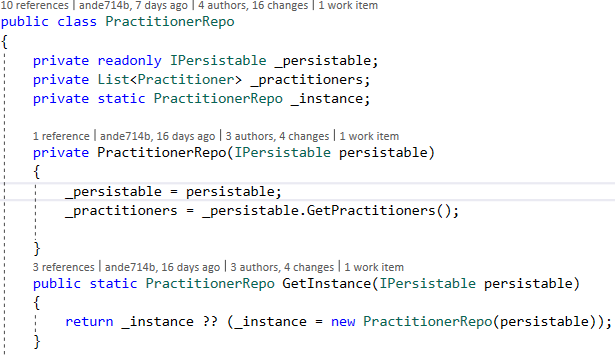
\includegraphics[width=\textwidth]{Singleton.png}
    \label{code:singleton}
\end{figure}

\subsubsection{Observer}
\label{observer}

Idéen med observermønstret er at skabe en fornuftig en-til-mange afhængigmed mellem objekter, så når et objekt ændrer tilstand får alle dens afhængige klasser en besked og opdateres automatisk.\cite{gangoffour}

Det bruges rigtig meget til at styre, hvordan et UI bliver opdateret, når programmet ændrer tilstand.

I C\# er der flere måder at implementere et observermønster: de mest udbredte måder er gennem 2 interfaces(et udgiver og et abonnent interface) eller ved hjælp af delegates.
I C\# findes en delegate, der hedder EventHandler, som normalt bruges, når man laver et observermønster vha delegates.

Som det kan ses på figur \ref{fig:ControllerObserverPattern} har vi implementeret vores observermønstre ved brug af EventHandler delegaten.
Vi har valgt at bruge delegates i stedet for interfaces, da vi så ikke behøver at lave og implementere to interfaces, men i stedet gør vi brug af værktøjer, der allerede eksisterer.
Derudover ville vi gerne få mere erfaring i at bruge delegates og events, da vi ikke har arbejdet lige så meget med det i løbet af året som med interfaces.

Som det kan ses på figur \ref{fig:ControllerObserverPattern} er vores Controller klasse både en udgiver og en abonnent.
Det er den nød til, da som beskrevet i afsnit \ref{facade}, er Controller en facade, og derfor kan vores UI ikke abonnere direkte ned til andre udgivere i vores applikationslag.

Vores UI abonnerer på vores controller, som abonnerer på vores appointmentrepo og clientrepo klasser.
På figur \ref{fig:ObserverObservermethod} kan det ses, at når controlleren får at vide, at der er sket en ændring i clientrepo eller appointmentrepo giver den sine abonnenter besked om det.



\begin{figure}[h]
    \caption{Controller observer mønster}
    \centering
        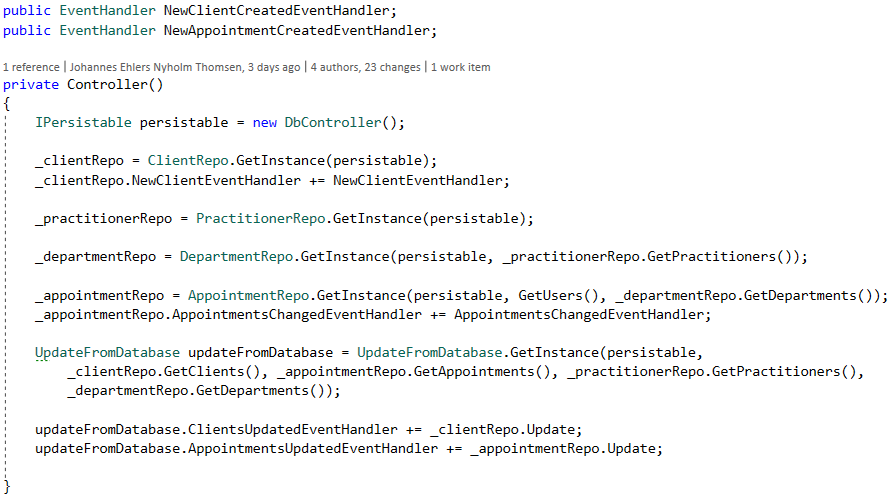
\includegraphics[width=\textwidth]{ControllerObserverPattern.png}
    \label{fig:ControllerObserverPattern}
\end{figure}

\begin{figure}[h]
    \caption{Controller abonnentmetoder.}
    \centering
        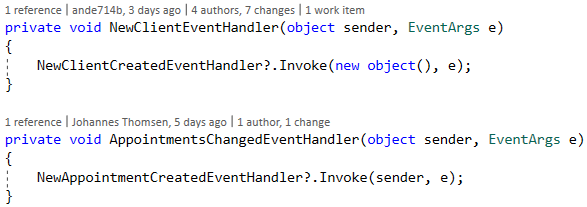
\includegraphics[width=\textwidth]{ObserverObservermethod.png}
    \label{fig:ObserverObservermethod}
\end{figure}

\subsection{GRASP}
\label{grasp}

TODO: DITTO MEN GRASP

\subsubsection{Controller}
\label{controller}
Vi gør brug af en controller til at facilitere kald fra UI'et, der kræver kald ned i applikations- og domænelaget.
Dette betyder, at vi indkapsulerer en systemoperation.
En systemoperation er noget, som en bruger af systemet ønsker at opnå, f.eks at booke en ny aftale.

Vi opnår så systemoperationen ved, at controlleren kalder de nødvendige metoder i resten af systemet.

Da vi, som nævnt i afsnit \ref{lagdeling}, har et applikationslag er det oplagt at bruge en controller til netop at give os det ønskede lag mellem UI og domæne.

Vores controller er også en facade mellem UI- og applikationslagene, se afsnit \ref{facade}.
